\documentclass[a4paper,10pt]{article}
%\usepackage[utf8x]{inputenc}
%\usepackage{czech}
\usepackage[utf8]{inputenc}
\usepackage[czech]{babel}
\usepackage{graphicx}

\title{Zpráva k~seminární úloze z~předmětu\\ Inteligentní robotika \\ {\small Závěrečná zpráva}}
\author{Filip Jareš, Lenka Mudrová}
\date{27.4.2011}

\begin{document}

\maketitle
\begin{figure}[!h]
	\centering
	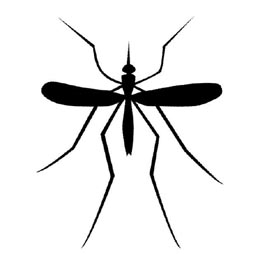
\includegraphics[width=0.4\columnwidth]{pics/mosquito}
	%\caption{}\label{fig:m}
\end{figure}
\newpage

\section{Popis úlohy}
		Řešená úloha je inspirována článkem Backyard star wars \cite{zadani}, který se zabývá problémem
		detekce komára ve venkovním prostředí a jeho sestřelení laserovým paprskem. 
		Pro školní účely byla tato myšlenka pozměněna, komár je nahrazen černým čtvercem, který se pohybuje na bílém
		pozadí monitoru, namísto laseru je pouze sledován kamerou.

		Poloha kamery se ovládá s použitím dvou modelářských serv a to  
		natočením okolo svislé osy (změnou azimutu) a natočením okolo vodorovné osy (změnou elevace). Cílem úlohy
		je řídit kameru tak, aby sledovala pohyb komára a zdokumentovala jeho „sestřel“
		sérií snímků, ve kterých je komár ve středu obrazu z~kamery – uprostřed
		„záměrného kříže“.

		

\section{Rozbor problému}
		Úloha se skládá z~několika oblastí, především je zde zastoupena oblast
		po\-čí\-ta\-čo\-vé\-ho vidění, kdy je nutné sejmout obrázek z~kamery, zpracovat ho a
		detekovat v~obraze komára. 
	        Další oblastí, která je zastoupena, je řízení. Celý
		program tvoří zpětnovazební regulační smyčku.
		Pro lepší funkci predikovat pohybu komára.  % FIXME: Tahle věta podle mě nezapadá dobře do okolních vět, takže moc nedává smysl.
		V~neposlední řadě je v~problému zastoupena robotika, kdy je potřeba pracovat se
		soustavou serv a počítat transformace souřadnic mezi obrazovkou a souřadným
		systémem serv.

		\subsection{Popis konstrukce soustavy}
		Použitá soustava je tvořena LCD monitorem s poměrem stran $4:3$ a kamerou umístěnou na pan-tilt jednotce \cite{kamera} .
		Obrázek \ref{fig:soustava} znázorňuje vzájemné umístění monitoru a kamery.
		Pan-tilt jednotka je tvořena dvěma modelářskými servomechanismy, které umožňují pohyb mezi $x-y stupni$.
		% FIXME: To je divná formulace s těmi x-y stupni. Raději popsat/zmínit osy rotace?
		%TODO: udelat obrazek

	       \subsection{Popis kamery a ovládání}
	       %TODO: popis

	       \subsection{Popis servo mechanismu a ovládání}
		%TODO: popis? Tady jen popsat tu jejich funkci nebo? Nejak nevim

\section{Změny specifikace}

\section{Řešení problému}

		Rámec programu je tvořen zpětnovazební regulační smyčkou pro řízení polohy
		kamery. Vstupem regulátoru je nejnovější získaný obrázek z~kamery a jeho
		výstupem je nová poloha kamery. Schématicky je to znázorněno na
		obrázku~\ref{fig:ridiciSystem}.  Před samotným výpočtem nové polohy kamery
		je vyhodnocen nově zís\-ka\-ný obraz. Postup jeho zpracování je znázorněn na
		obrázku~\ref{fig:zpracovaniObrazu}.  Nejprve je určena poloha komára v~obraze
		(funkce \textit{findMosquitoInImage}) v~pixelových sou\-řad\-ni\-cích. Na základě odchylky
		této polohy od středu obrázku potom funkce
		\textit{mos\-quito\-Px\-PositionToAzimuthAndElevation} počítá odhad úhlů, o~které je
		komár vy\-chý\-len od optické osy kamery. Pro urychlení celé smyčky jsou data pouze
		ukládána, nikoliv zobrazována. Uživatel si snadno tato data přehraje offline.

		\begin{figure}[!h]
			\centering
			 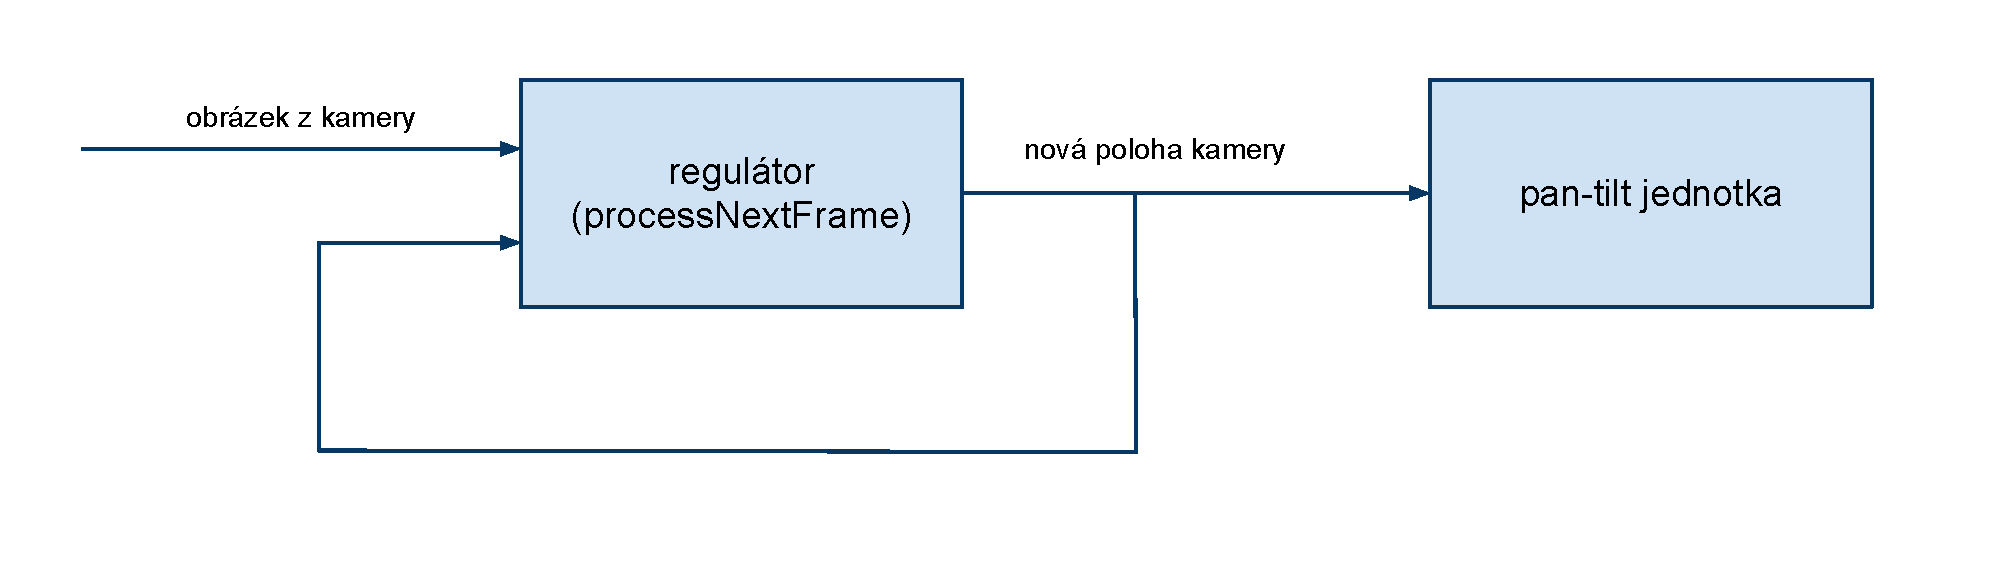
\includegraphics[width=1\columnwidth]{pics/schema_ridiciho_systemu}
			 \caption{Schéma řídícího systému}\label{fig:ridiciSystem}
		\end{figure}

\section{Implementace}

\bibliographystyle{splncs03}
\bibliography{report}

\end{document}
 
